\documentclass[11pt]{article}
\usepackage[utf8x]{inputenc}
\usepackage{amsmath}
\usepackage{graphicx}
\usepackage{float}
\usepackage{dsfont}
\usepackage{amsfonts}
\usepackage{lipsum}
\usepackage{epstopdf}
\usepackage[T1]{fontenc}
\usepackage[colorinlistoftodos]{todonotes}
\usepackage[left=2cm,right= 2cm,top=3cm,bottom=2.5cm,a4paper]{geometry}
\usepackage{listings}
\usepackage{multicol}
\usepackage{fancyhdr}
\usepackage{caption}
\usepackage{cite}
\usepackage{cleveref}
\usepackage{siunitx}
\setlength{\columnsep}{1cm}
\setlength{\parindent}{0pt}
\newcommand{\deriv}{\mathrm{d}}
\lstset{
    language=R,
    basicstyle=\scriptsize\ttfamily,
    commentstyle=\ttfamily\color{red},
    numbers=left,
    numberstyle=\ttfamily\color{blue}\footnotesize,
    stepnumber=1,
    numbersep=5pt,
    backgroundcolor=\color{white},
    showspaces=false,
    showstringspaces=false,
    showtabs=false,
    frame=single,
    tabsize=2,
    captionpos=b,
    breaklines=true,
    breakatwhitespace=false,
    title=\lstname,
    escapeinside={},
    keywordstyle={},
    morekeywords={}
}

\pagestyle{fancy}
\fancyhf{}
\rhead{PH370 Physics Labs}
\lhead{LLR.1 - Rotation Rate of Planet Mercury}
\rfoot{-\thepage\centering-}

\begin{document}
\begin{titlepage}

\newgeometry{left=1.5in,right=1.5in,top=2.5in,bottom=2.5in}
\newcommand{\HRule}{\rule{\linewidth}{0.5mm}}

\begin{centering} 
 
%------------------------------------------------------------------------
%	HEADING SECTIONS
%------------------------------------------------------------------------


\includegraphics[scale=0.4]{Uni_of_Kent_Logo.png}\\[1cm]

%------------------------------------------------------------------------
%	TITLE SECTION
%------------------------------------------------------------------------

\HRule \\[0.4cm]
\textsc{\large Astronomy, Space Science and Astrophysics}\\[0.4cm]
{\Huge \bfseries Rotation Rate of \\ [0.5cm] Planet Mercury}\\[0.4cm]
\HRule \\[1.0cm]

%------------------------------------------------------------------------
%	DATE SECTION
%------------------------------------------------------------------------

\textsc{\Large Stage 1 - PH370 Physics Labs}\\[0.5cm] 
{\large Monday 29th Jan - 5th Feb 2018}\\[1.0cm]

%------------------------------------------------------------------------
%	AUTHOR SECTION
%------------------------------------------------------------------------

\begin{minipage}{0.625\textwidth}
\centering

\emph{\large Report Author:} \large Lukasz R Tomaszewski \\ [0.2cm]
\emph{\large Lab Partner:} \large Jordan Thijssen \\

\end{minipage}\\[2cm]

\vfill
\end{centering} 
\end{titlepage}

%------------------------------------------------------------------------
%------------------------------------------------------------------------
%	CONTENTS  
%------------------------------------------------------------------------
%------------------------------------------------------------------------

\newpage
\begin{titlepage}
\newgeometry{left=1in,right=1in,top=1in,bottom=1in}
\tableofcontents
\end{titlepage}

%-----------------------------------------------------------------------
%-----------------------------------------------------------------------
%	ABSTRACT
%-----------------------------------------------------------------------
%-----------------------------------------------------------------------

\begin{multicols}{2}

\section{Abstract}

The aim of this experiment is to find the rotational velocity of planet Mercury through firing short electromagnetic radiation pulses to Mercury and receiving the reflected pulses back off the planets surface. The experiment was repeated 3 times using present date, a date of Mercury’s inferior conjunction and a date of Mercury’s greatest-eastern elongation. The final 3 answers weren't spot on correct due to human error but was close therefore the underlying physics does work and is proved throughout this report.

%-----------------------------------------------------------------------
%-----------------------------------------------------------------------
%	INTRODUCTION
%-----------------------------------------------------------------------
%-----------------------------------------------------------------------

\section{Introduction}

This experiments main objective is to use electromagnetic waves to determine the rotational rate of planet Mercury. This was done by firing a sequence of short electromagnetic radiation pulses to three of many of planet Mercury’s positions in orbit around the sun; random position on present date where Mercury is on the far side of the sun to Earth, inferior conjunction where Mercury is closest to Earth and the greatest-eastern elongation where Mercury is on the furthest eastern side of the Sun in relation to Earth. \\

Using the frequency data graph received from the electromagnetic radiation pulses that reflected off the planet Mercury's surface closest to Earth, highlighted to echoes; the lower frequency echo (rotational velocity component away from Earth) and the higher frequency echo (rotational velocity component towards Earth). The echoes were then implemented into a series of formulas highlighted in \cite{LLR.1-2018}, the results produced in \cref{Data Collected} shows all three experiments; present date, inferior conjunction \& greatest-eastern elongation.

%-----------------------------------------------------------------------
%-----------------------------------------------------------------------
%	AIMS & EQUIPMENT
%-----------------------------------------------------------------------
%-----------------------------------------------------------------------

\section{Aims \& Equipment}

%-----------------------------------------------------------------------
%	APPARTUS
%-----------------------------------------------------------------------

\subsection{Apparatus}

\begin{itemize}
	\item CLEA Software
\end{itemize}

%-----------------------------------------------------------------------
%	DATA COLLECTED
%-----------------------------------------------------------------------

\subsection{Data Collected}\label{Data Collected}

\begin{itemize}
	\item Outgoing frequency
	\item Delay distance
    \item Distance parallel to Earth
    \item Distance perpendicular to Earth
    \item Shift in rotational velocity frequency
    \item Shift in frequency due to echo
	\item Rotational velocity of Mercury
    \item Equatorial rotational velocity
    \item Rotational period of Mercury
    \item Inferior conjunction
    \item Greatest-Eastern conjunction
    \item Greatest-Western conjunction
\end{itemize}

%-----------------------------------------------------------------------
%	RISK ASSESSMENT
%-----------------------------------------------------------------------

\subsection{Risk Assessment}

When performing any physical experiment, there are risks involved, in relation to this experiment there are ergonomic risks where physical fatigue aches \& pains in joints \& limbs. Lighting has the potential to cause glare thus will cause eye strain and headaches, upper limb disorders include effects such as tendinitis and carpal tunnel syndrome. \\

As the time duration of this experiment is 3-4 hours long, controlling these hazards and preventing them turning into risks is a priority. A computer is required to run the software thus swapping the operator of the computer regularly will reduce the risk of a single operator eye strain \& headaches, during this stage the operators can stretch their legs to prevent upper limb disorders. In prevention of electrical hazards, the computer had a green PAT (portable appliance test) sticker which states its safe to use. 

%-----------------------------------------------------------------------
%-----------------------------------------------------------------------
%	EXPERIMENTAL PROCEDURE
%-----------------------------------------------------------------------
%-----------------------------------------------------------------------

\section{Experimental Procedure}

%-----------------------------------------------------------------------
%	PHYSICS BEHIND THE EXPERIMENT
%-----------------------------------------------------------------------

\subsection{Physics Behind the Experiment} \label{Physics Behind the Experiment}

\begin{figure}[H]
\centering
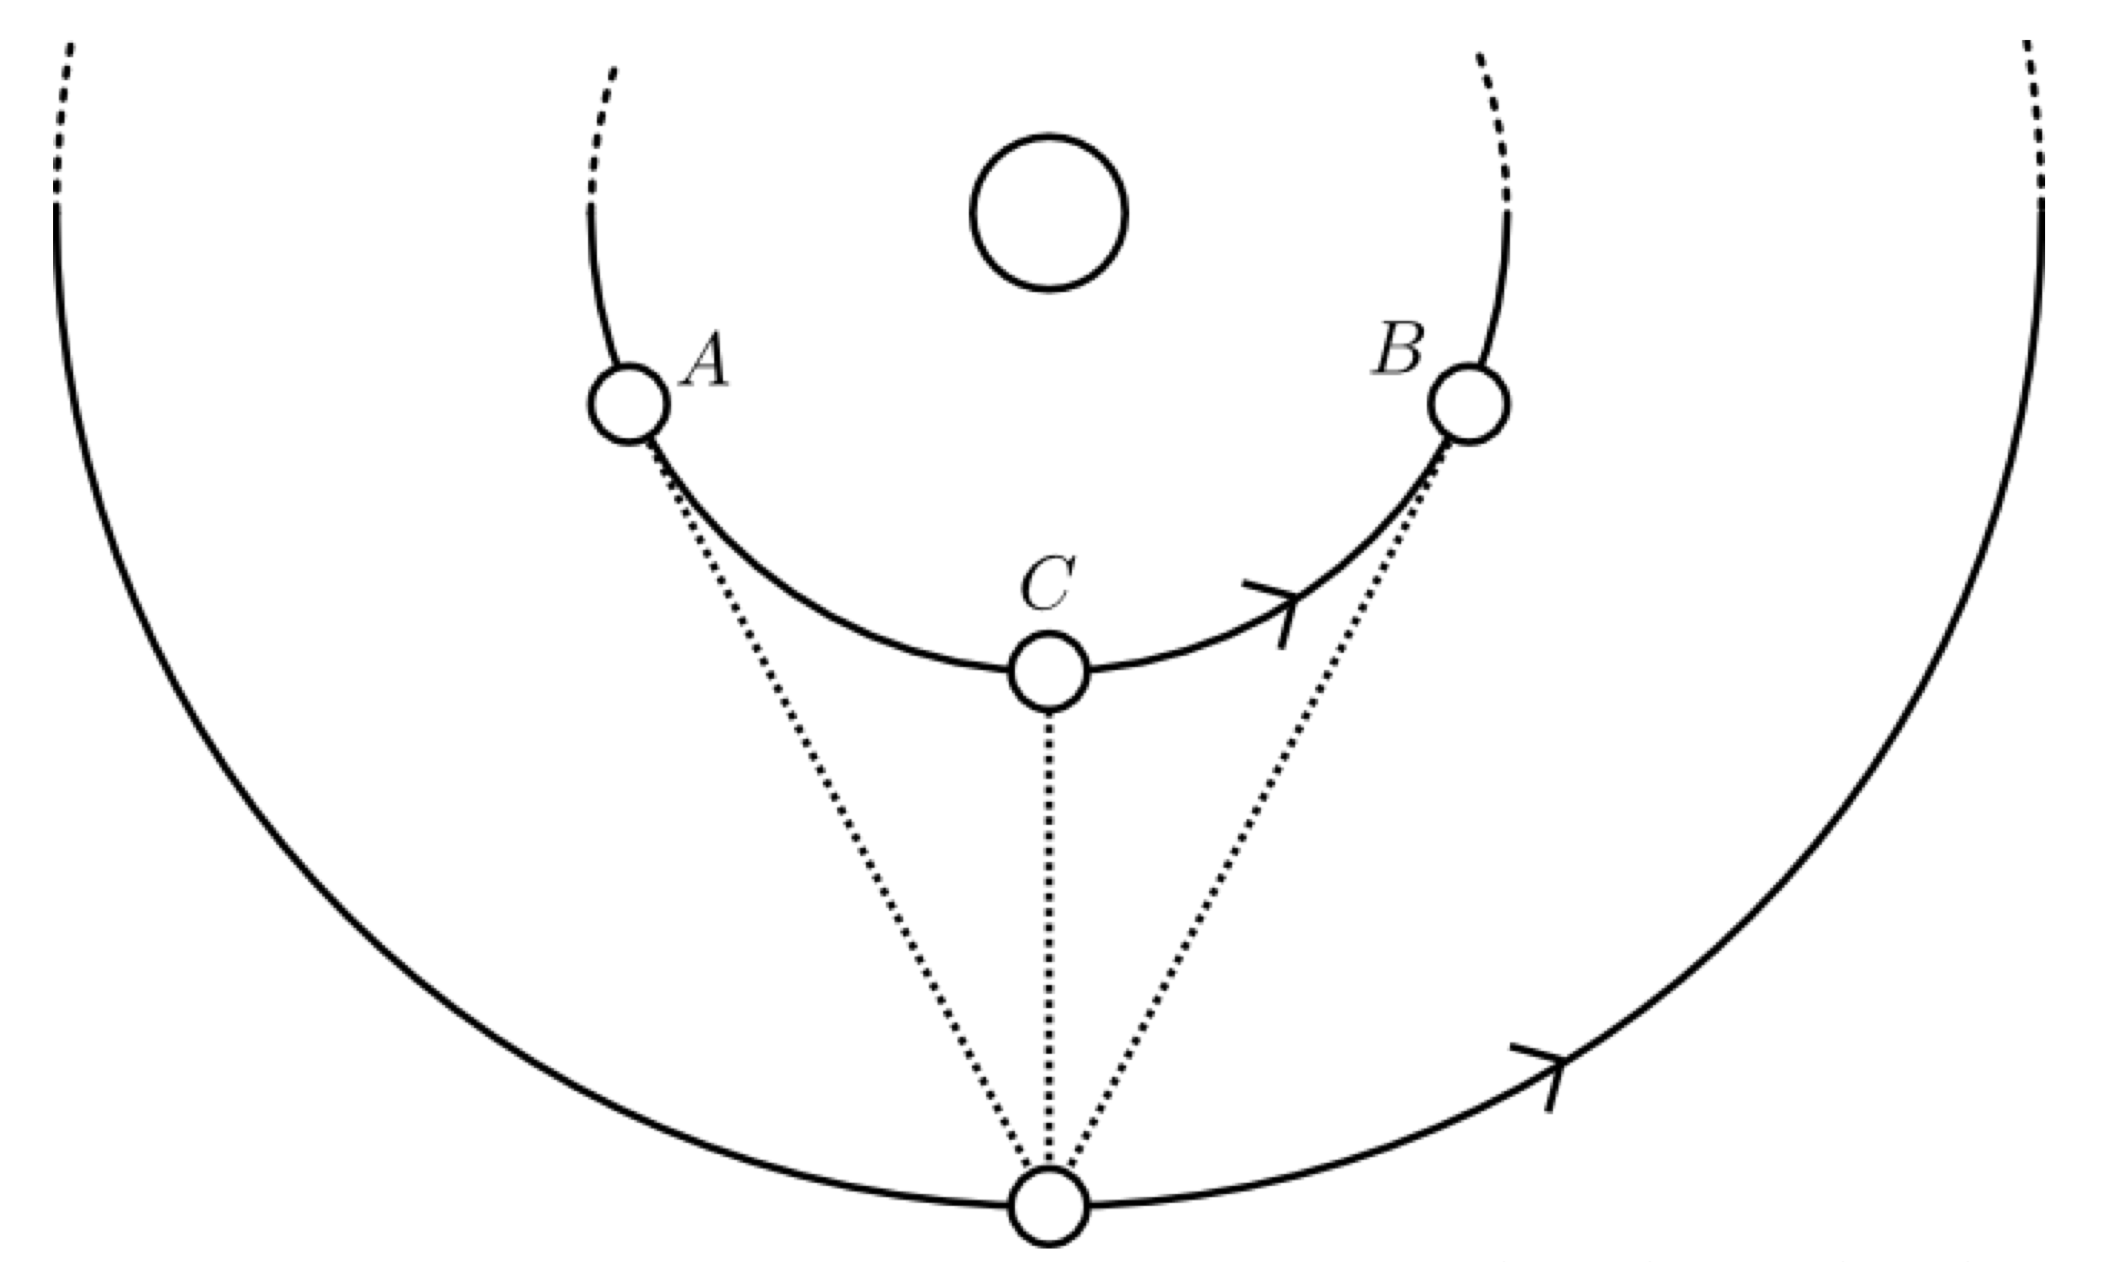
\includegraphics[scale=0.18]{Planetary_Positions.png}
\caption{Mercury's position in orbit of the sun in relation to Earth.}
\label{Planetary Positions}
\end{figure}

As shown in \cref{Planetary Positions} which is located in \cite{LLR.1-2018}, Mercury's orbit around the sun is much shorter than Earth's, therefore the period of rotation will be much less than Earth's. In this experiment, a series of short electromagnetic radiation pulses of known frequency will be fired and sent in a direct path to mercury and the received pulse which reflected off Mercury's surface will be plot a graph (frequency value against frequency intensity). The travel time of the pulses in each stage of this experiment will vary depending on the distance between Mercury and Earth. \\

A notable statement to make is that the outgoing pulse that is sent, the entire pulse will not all hit the planet Mercury's surface due the fact the pulse will stretch to cover a larger area but the part of the pulse that does hit the planets surface will hit the surface at different times as show in \cref{Planet freq target} which is located in \cite{LLR.1-2018}. \\

\begin{figure}[H]
\centering
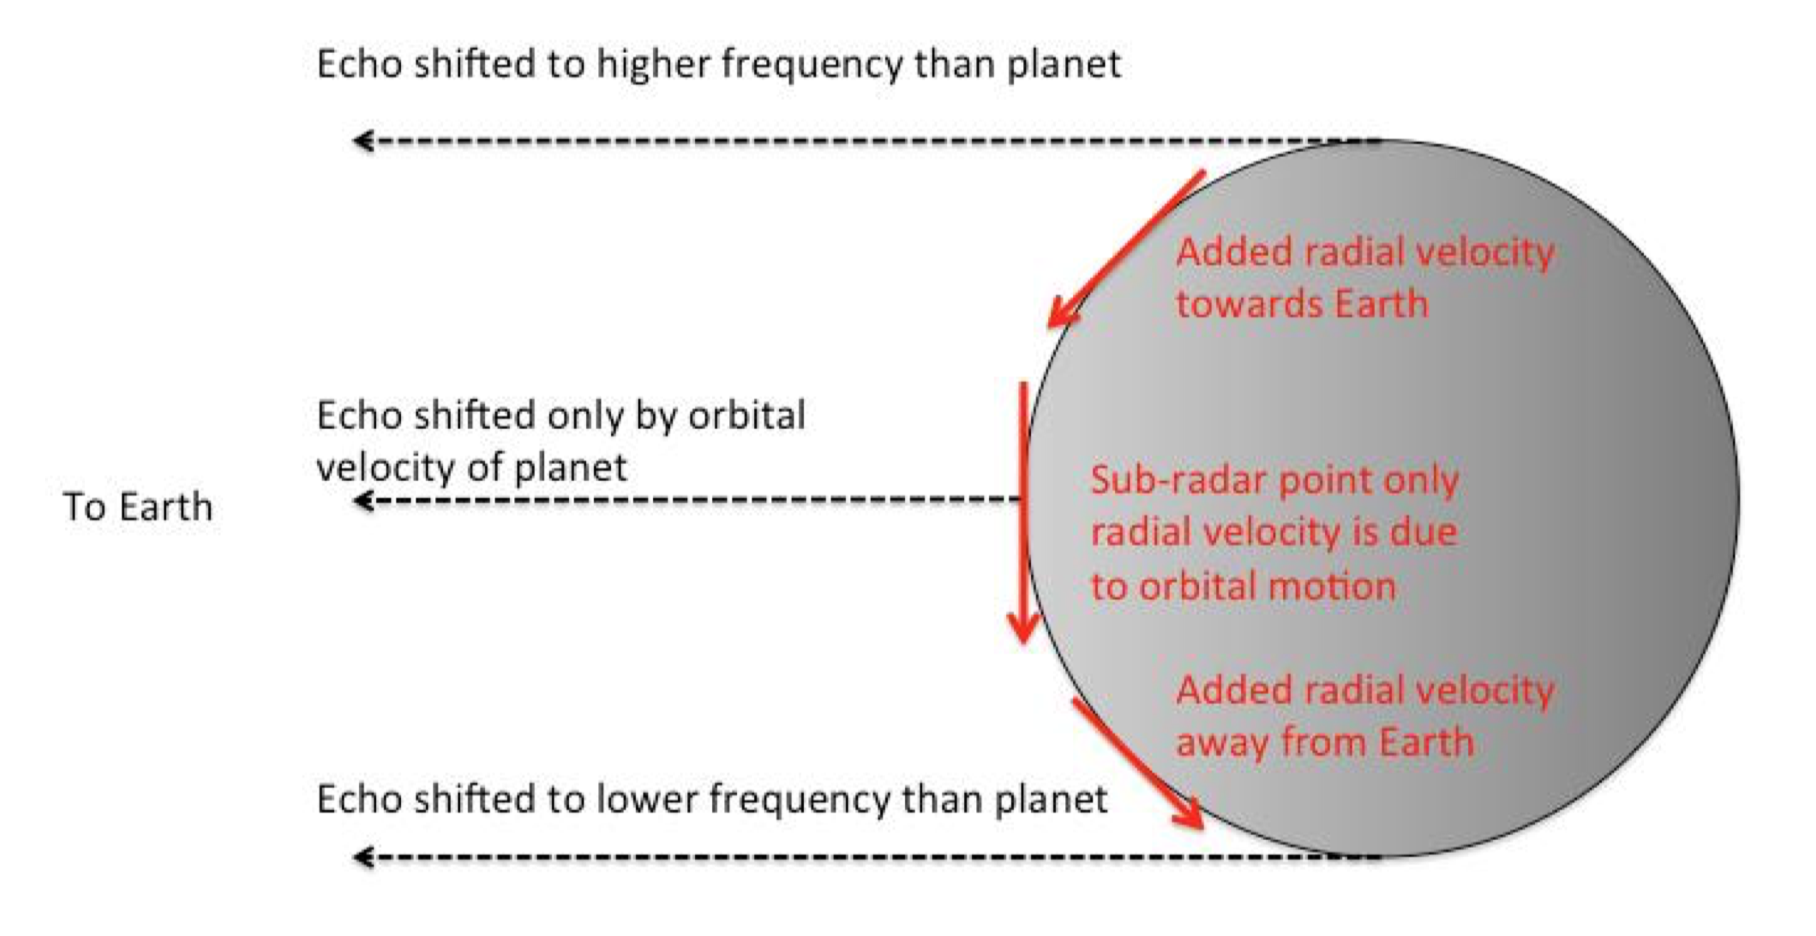
\includegraphics[scale=0.25]{Planet_freq_target.png}
\caption{The sub radar point and radial velocities of the planets surface.}
\label{Planet freq target}
\end{figure}

Due to Doppler effect, the returning echoes are slightly higher and lower, the returning echo received of the radial velocity towards Earth is a slightly higher frequency and the the returning echo received of the radial velocity away Earth is a slightly lower frequency. But due to the knowledge of the Doppler effect, the application can be applied. \\

\begin{figure}[H]
\centering
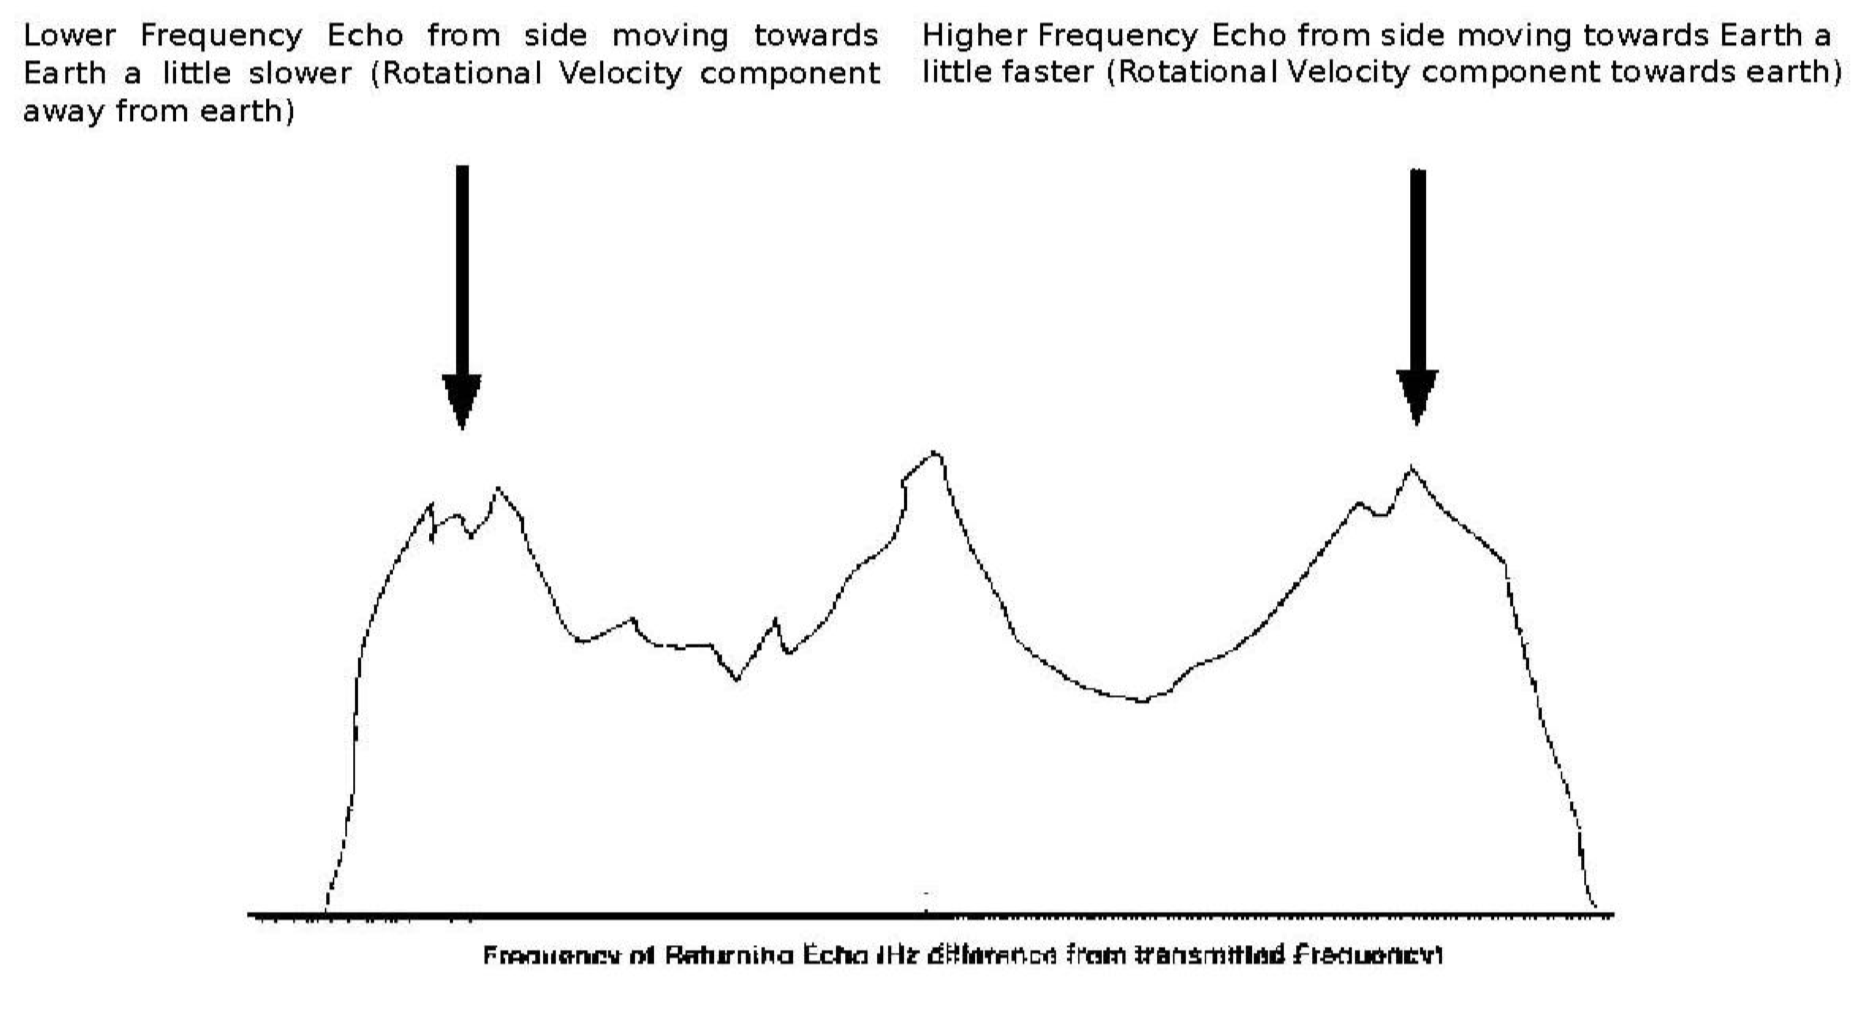
\includegraphics[scale=0.24]{Graph_Diagram.png}
\caption{The received pulses graph.}
\label{Graph Diagram}
\end{figure}

\cref{Graph Diagram} which located in \cite{LLR.1-2018} shows that the left peak is Mercury's side moving towards Earth and the right peak is Mercury's side moving away from Earth and the middle peak being the sub radar point as shown in \cref{Planet freq target}. \\

\begin{figure}[H]
\centering
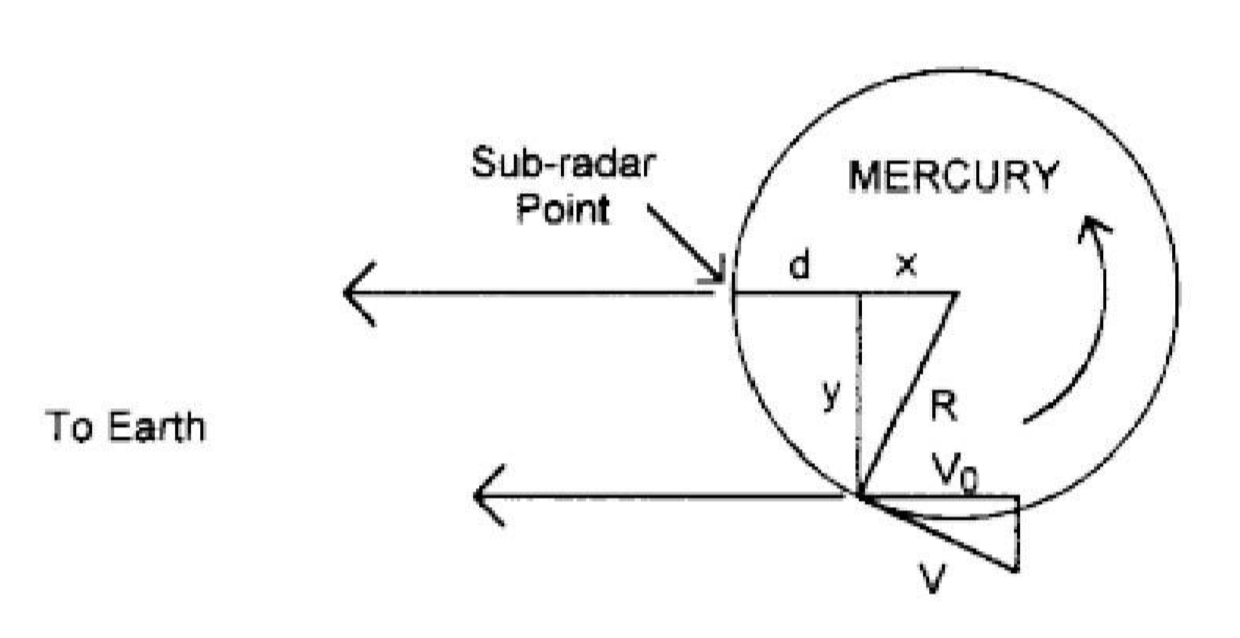
\includegraphics[scale=0.35]{d_x_y_Diagram.png}
\caption{Geometrical view of the calculations within this experiment.}
\label{d_x_y Diagram}
\end{figure}

Using the geometrical view in \cref{d_x_y Diagram} which located in \cite{LLR.1-2018}, calculations can be made with the data received back from the electromagnetic pulse which are highlighted in \cref{Results Disscussion} but d, x and y can be calculated without any received data but are of paramount importance in later equations. These geometrical parameters: d, x and y are located in \cref{Geometrical Parameters} of this report.

%-----------------------------------------------------------------------
%	PRESENT DATE
%-----------------------------------------------------------------------

\subsection{Present Date}\label{Present Date}

\begin{figure}[H]
\centering
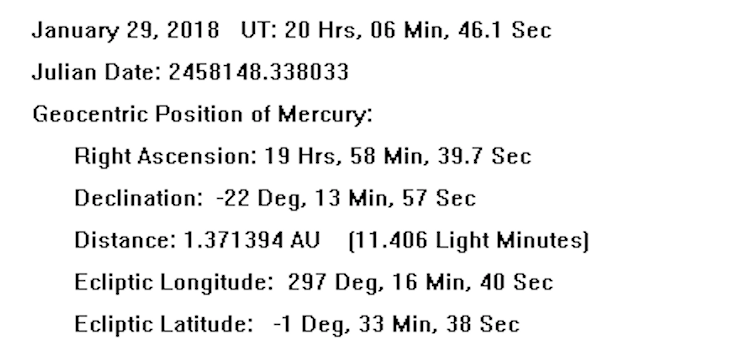
\includegraphics[scale=0.6]{Present_Images.png/Data_Set.png}
\caption{The data set used for the present date stage of this experiment, showing the astronomical measurements of Mercury in relation to Earth.}
\label{1-Data Set}
\end{figure}

In the first stage of this experiment, using the CLEA software, and todays date a series of short electromagnetic radiation pulses were fired from Earth to Mercury, with the position of Mercury in relation to the Sun and Earth, as shown in \cref{1-Data Set}. \\

\begin{figure}[H]
\centering
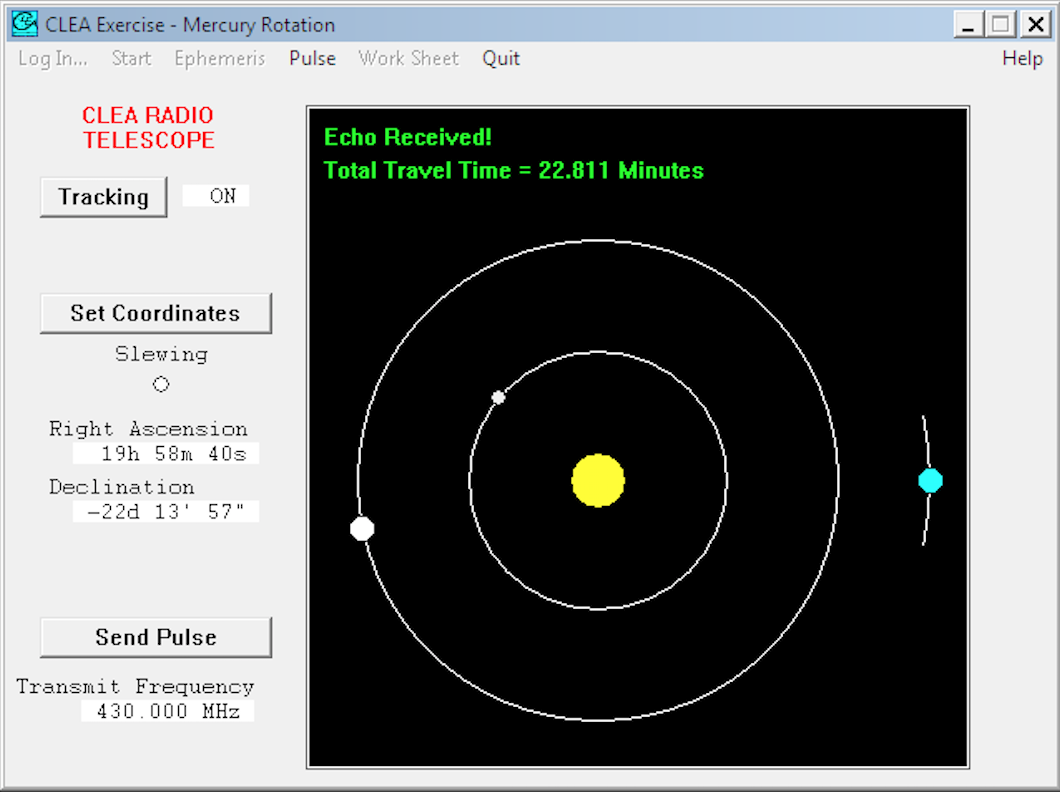
\includegraphics[scale=0.4]{Present_Images.png/CLEA_Software.png}
\caption{Screen shot of the CLEA software for the present date stage of this experiment showing the positions of Earth and Mercury in relation to the Sun.}
\label{1-CLEA Software}
\end{figure}

While \cref{1-CLEA Software} shows the positions of Mercury in relation to Earth around the Sun, as clearly shown this pulse out of all 3, this was had the longest travel time as Mercury was on the other side of the Sun in relation to Earth. After the 22.811 minutes the received pulse hit Earth and the experiment continued, the frequency were picked and the list of equations were filled to give a final answer to the rotational rate of planet Mercury which are all highlighted in \cref{Present date data}. 

%-----------------------------------------------------------------------
%	INFERIOR CONJUNCTION
%-----------------------------------------------------------------------

\subsection{Inferior Conjunction}

\begin{figure}[H]
\centering
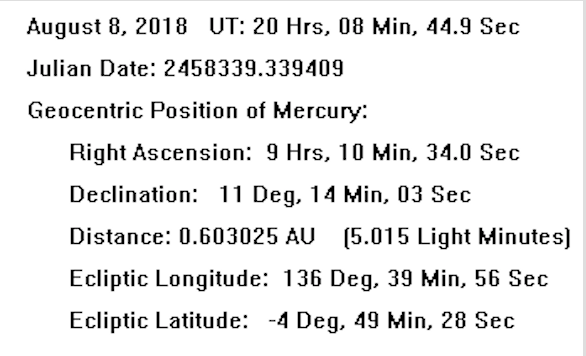
\includegraphics[scale=0.6]{Inferior_Images.png/Data_Set.png}
\caption{The data set used for the inferior conjunction stage of this experiment, showing the astronomical measurements of Mercury in relation to Earth.}
\label{2-Data Set}
\end{figure}

In the second stage of this experiment, much like in the first stage  using the CLEA software, inputting a date of one of this years inferior conjunctions of Mercury in relation to Earth which was found at \cite{astropixels.com}, the series of short electromagnetic radiation pulses were fired from Earth to Mercury again, with the position of Mercury in relation to the Sun and Earth, as shown in \cref{2-Data Set}. \\

\begin{figure}[H]
\centering
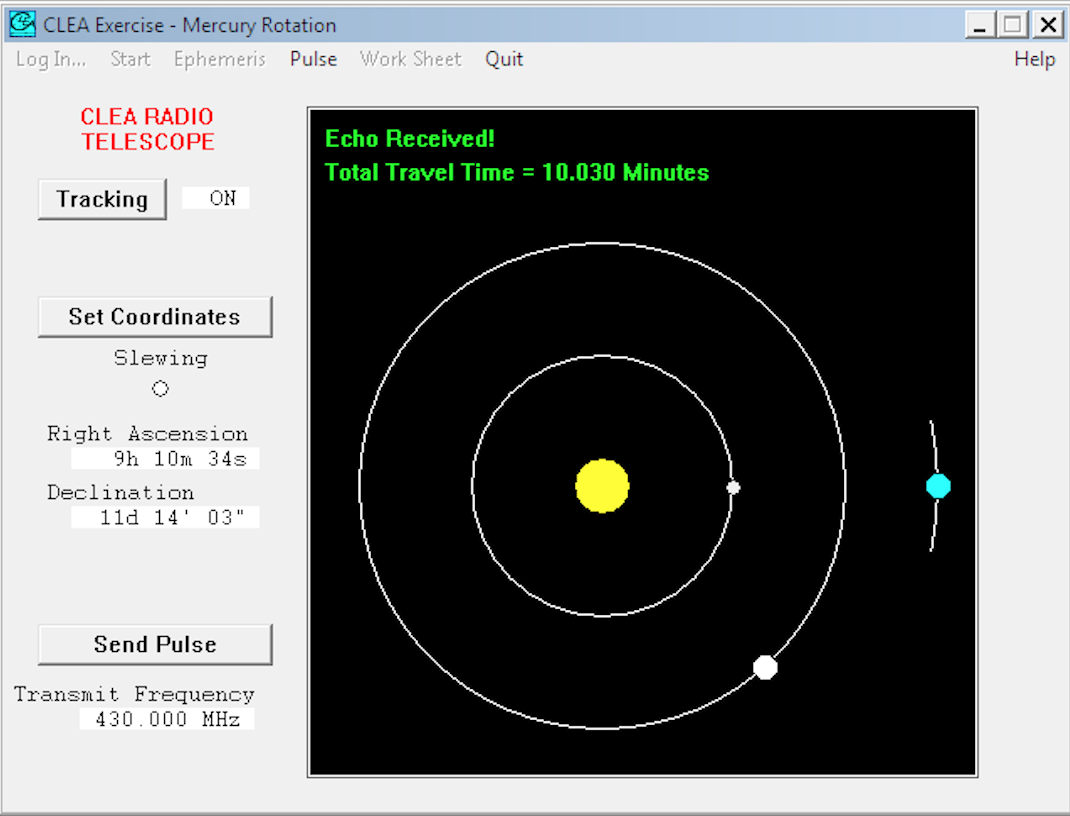
\includegraphics[scale=0.4]{Inferior_Images.png/CLEA_Software.png}
\caption{Screen shot of the CLEA software for the inferior conjunction stage of this experiment showing the positions of Earth and Mercury in relation to the Sun.}
\label{2-CLEA Software}
\end{figure}

While \cref{2-CLEA Software} shows the positions of Mercury in relation to Earth around the Sun. After the 10.030 minutes the received pulse hit Earth and the experiment continued much like \cref{Present Date} and the data was collected as shown in \cref{Inferior Conjunction}. 

%-----------------------------------------------------------------------
%	GREATEST_EASTERN ELONGATION
%-----------------------------------------------------------------------

\subsection{Greatest-Eastern Elongation}

\begin{figure}[H]
\centering
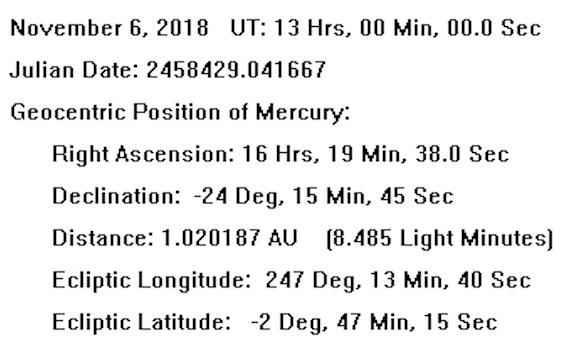
\includegraphics[scale=0.6]{Great-East_Images.png/Data_Set.png}
\caption{The data set used for the greatest-eastern elongation stage of this experiment, showing the astronomical measurements of Mercury in relation to Earth.}
\label{3-Data Set}
\end{figure}

In the third stage of this experiment, much like in the first \& second stage, inputting a date of one of this years greatest-eastern elongations of Mercury in relation to Earth which was found at \cite{astropixels.com} into the CLEA software, the series pulses were fired from Earth to Mercury again, with the position of Mercury in relation to the Sun and Earth, as shown in \cref{3-Data Set}. \\

\begin{figure}[H]
\centering
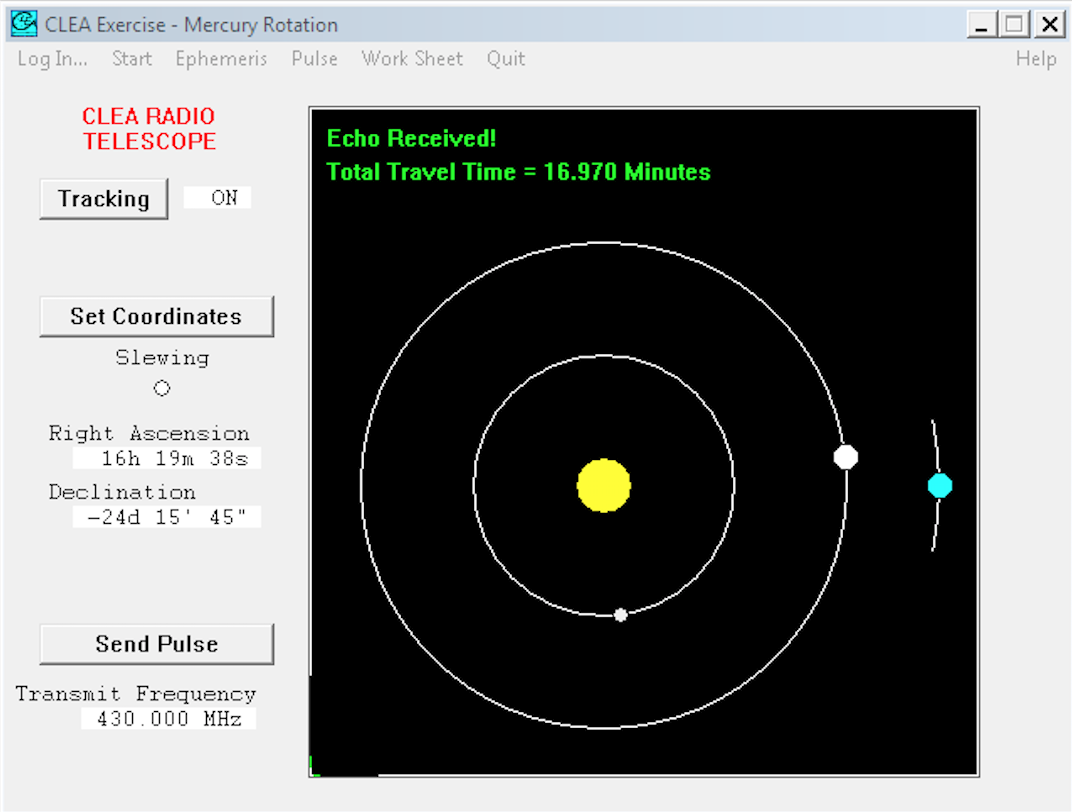
\includegraphics[scale=0.4]{Great-East_Images.png/CLEA_Software.png}
\caption{Screen shot of the CLEA software for the greatest-eastern elongation stage of this experiment showing the positions of Earth and Mercury in relation to the Sun.}
\label{3-CLEA Software}
\end{figure}

While \cref{3-CLEA Software} shows the positions of Mercury in relation to Earth around the Sun. After the 16.970 minutes the received pulse hit Earth and the experiment continued much like \cref{Present Date} \& \cref{Inferior Conjunction} and the data was collected as shown in \cref{Greatest-Eastern Elongation}. \\

%-----------------------------------------------------------------------
%-----------------------------------------------------------------------
%	RESULT & DISSCUSSION
%-----------------------------------------------------------------------
%-----------------------------------------------------------------------

\section{Results \& Disscussion}\label{Results Disscussion}

%-----------------------------------------------------------------------
%	SET PARAMETERS
%-----------------------------------------------------------------------

\subsection{Geometrical Parameters}\label{Geometrical Parameters}

\addtolength\abovedisplayskip{-0.5\baselineskip}
\addtolength\belowdisplayskip{-0.5\baselineskip}

\subsubsection{Delay Distance}

\begin{equation} \label{Delay distance equation}
{d = \dfrac{c \Delta t }{2}}
\end{equation}

\begin{equation*}
\begin{split}
&\text{Where;} \\
&\text{Speed of Light} \Rightarrow c=3_{\times10^8} \\
&\text{Change in Time} \Rightarrow \Delta t = \text{\cref{Physics Behind the Experiment}} \\
\end{split}
\end{equation*} \\

Using \cref{Delay distance equation}, the delay distance parameter was calculated for further use in the present date experiment (\cref{Present date data}), inferior conjunction experiment (\cref{Inferior Conjunction}) and greatest-eastern elongation experiment (\cref{Greatest-Eastern Elongation}). 

\begin{equation}\label{Delay distance parameter}
\begin{split}
&T + 120 \Rightarrow {d = \dfrac{3_{\times10^8} \times 120_{\times10^{-6}}}{2}=18_{\times10^3}} \\       
\\
&T + 210 \Rightarrow {d = \dfrac{3_{\times10^8} \times 210_{\times10^{-6}}}{2}=31.5_{\times10^3}} \\
\\
&T + 300 \Rightarrow {d = \dfrac{3_{\times10^8} \times 300_{\times10^{-6}}}{2}=45_{\times10^3}} \\
\\
&T + 390 \Rightarrow {d = \dfrac{3_{\times10^8} \times 390_{\times10^{-6}}}{2}=58.5_{\times10^3}} \\
\\
\end{split}
\end{equation}

%-----------------------------------------------------------------------

\subsubsection{Distance parallel to our line of sight}

\begin{equation} \label{Distance parallel to our line of sight equation}
{x = R_{Merc} - d}
\end{equation}

\begin{equation*}
\begin{split}
&\text{Where;} \\
&\text{Radius of Mercury} \Rightarrow {R_{Merc}}=2.24_{\times10^6} \\
&\text{Delay Distance} \Rightarrow d = \cref{Delay distance equation} \\
\end{split}
\end{equation*}\\

Using \cref{Distance parallel to our line of sight equation}, the distance parallel to our line of sight parameter was calculated for further use in the present date experiment (\cref{Present date data}), inferior conjunction experiment (\cref{Inferior Conjunction}) and greatest-eastern elongation experiment (\cref{Greatest-Eastern Elongation}). 

\begin{equation} \label{Distance parallel to our line of sight parameter}
\begin{split}
&T + 120 \Rightarrow {x= 2.24_{\times10^6}-18_{\times10^3}=2.402_{\times10^6}} \\
\\
&T + 210 \Rightarrow {x= 2.24_{\times10^6}-31.5_{\times10^3}=2.3885_{\times10^6}} \\
\\
&T + 300 \Rightarrow {x= 2.24_{\times10^6}-45_{\times10^3}=2.375_{\times10^6}} \\
\\
&T + 390 \Rightarrow {x= 2.24_{\times10^6}-58.5_{\times10^3}=2.3615_{\times10^6}} \\
\\
\end{split}
\end{equation}

%-----------------------------------------------------------------------

\subsubsection{Distance perpendicular to our line of sight}

\begin{equation} \label{Distance perpendicular to our line of sight equation}
{y = (R_{Merc}^{2} - x^{2})^{\dfrac{1}{2}}}
\end{equation}

\begin{equation*}
\begin{split}
&\text{Where;} \\
&\text{Radius of Mercury} \Rightarrow {R_{Merc}}=2.24_{\times10^6} \\
&\text{Distance parallel to our line of sight} \Rightarrow \\
& x= \cref{Distance parallel to our line of sight equation} \\
\end{split}
\end{equation*} \\

Using \cref{Distance perpendicular to our line of sight equation}, the distance perpendicular to our line of sight parameter was calculated for further use in the present date experiment (\cref{Present date data}), inferior conjunction experiment (\cref{Inferior Conjunction}) and greatest-eastern elongation experiment (\cref{Greatest-Eastern Elongation}). 

\begin{equation}\label{Distance perpendicular to our line of sight parameter}
\begin{split}
&T + 120 \Rightarrow {y=((2.24_{\times10^6})^{2} - (2.22_{\times10^6})^{2})^{\dfrac{1}{2}}} \\
&=294.612_{\times10^3} \\
\\
&T + 210 \Rightarrow {y=((2.24_{\times10^6})^{2} - (2.21_{\times10^6})^{2})^{\dfrac{1}{2}}} \\ 
&=389.189_{\times10^3} \\
\\
&T + 300 \Rightarrow {y=((2.24_{\times10^6})^{2} - (2.20_{\times10^6})^{2})^{\dfrac{1}{2}}} \\ 
&=464.516_{\times10^3} \\
\\
&T + 390 \Rightarrow {y=((2.24_{\times10^6})^{2} - (2.18_{\times10^6})^{2})^{\dfrac{1}{2}}} \\ 
&=528.883_{\times10^3} \\
\\
\end{split}
\end{equation}

%-----------------------------------------------------------------------
%	PRESENT DATE
%-----------------------------------------------------------------------

\subsection{Present Date}\label{Present date data}

Comparing the appearance of the received pulse \cref{1-Recieved Pulse} to the initial pulse \cref{1-Outgoing Pulse}, clearly shows it is broader than the initial pulse. The smooth gradient climb leading up to the sub-radar point which states the frequency shift had greater intensity as it hit the sub-radar point. A notable difference is that \cref{1-Recieved Pulse} is around 45,000Hz lower than the initial frequency.\\

The following \cref{1-T+120}, \cref{1-T+210}, \cref{1-T+300} \& \cref{1-T+390} graphs show the pulses received at 90 second intervals, apart from \cref{1-T+120} which is at a 120 second interval from \cref{1-Recieved Pulse}.

\subsubsection{Received Pulses Graphs}\label{Present Graphs}

\begin{figure}[H]
\centering
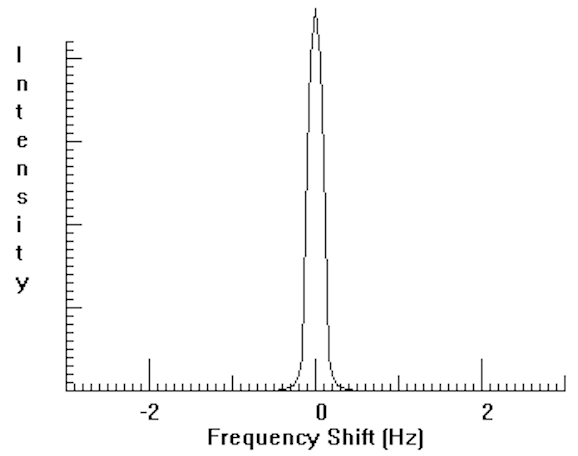
\includegraphics[scale=0.7]{Present_Images.png/1_-_Outgoing_Pulse.png}
\caption{Outgoing pulse of the electromagnetic signal.}
\label{1-Outgoing Pulse}
\end{figure}

\begin{figure}[H]
\centering
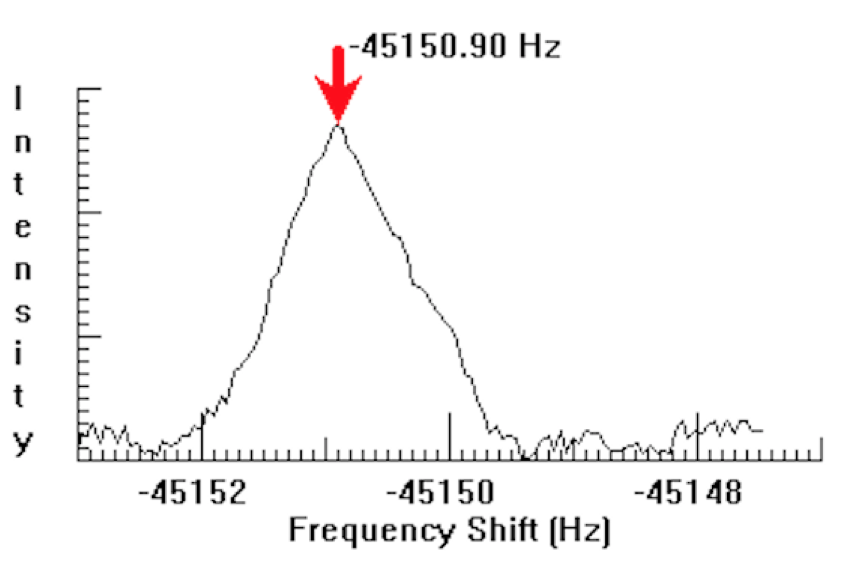
\includegraphics[scale=0.5]{Present_Images.png/1_-_T.png}
\caption{Received pulse of the electromagnetic signal.}
\label{1-Recieved Pulse}
\end{figure}

\begin{figure}[H]
\centering
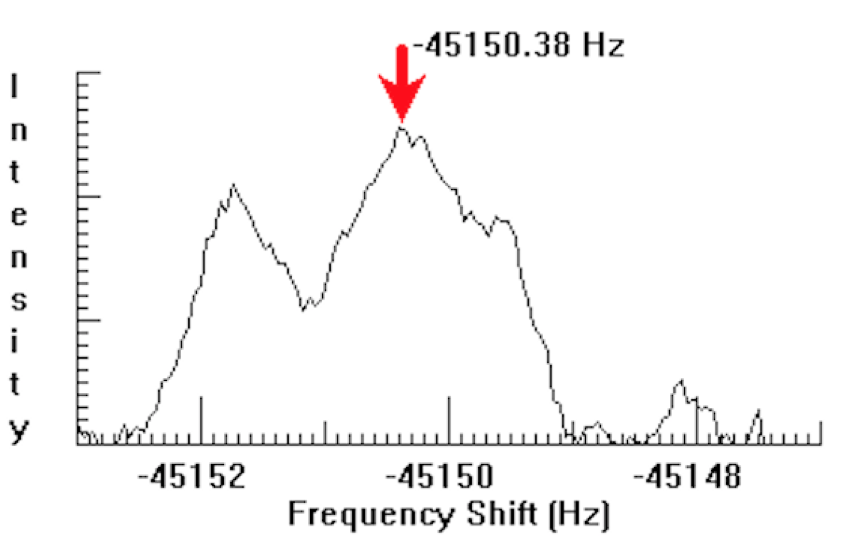
\includegraphics[scale=0.5]{Present_Images.png/1_-_T+120ms.png}
\caption{T+120s interval of the electromagnetic signal from the received pulse.}
\label{1-T+120}
\end{figure}

\begin{figure}[H]
\centering
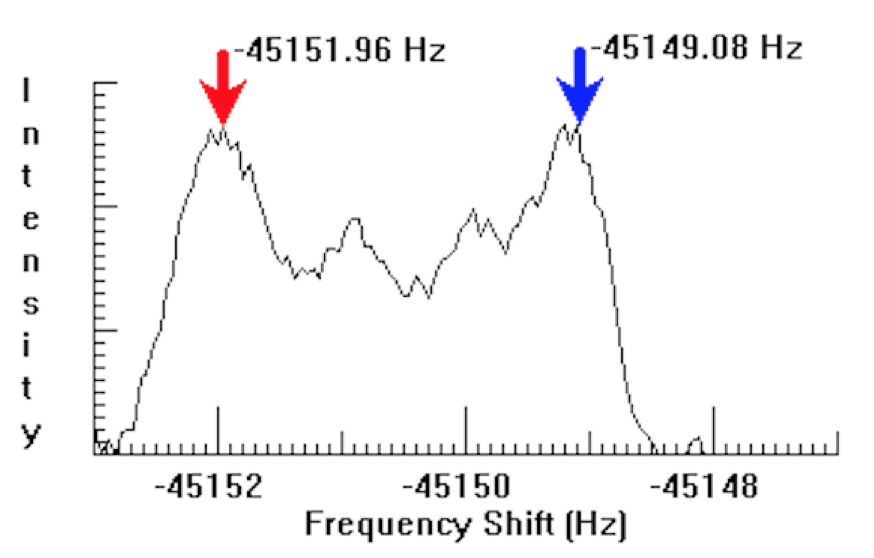
\includegraphics[scale=0.5]{Present_Images.png/1_-_T+210ms.png}
\caption{T+210s interval of the electromagnetic signal from the received pulse.}
\label{1-T+210}
\end{figure}

\begin{figure}[H]
\centering
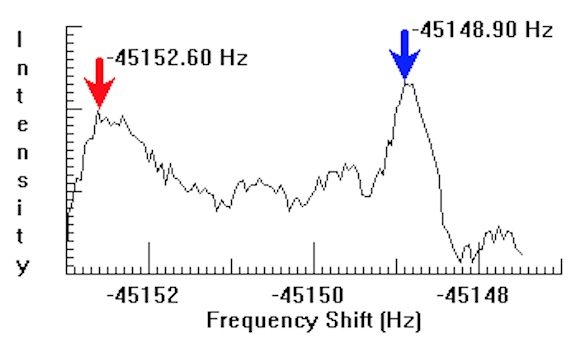
\includegraphics[scale=0.7]{Present_Images.png/1_-_T+300ms.png}
\caption{T+300s interval of the electromagnetic signal from the received pulse.}
\label{1-T+300}
\end{figure}

\begin{figure}[H]
\centering
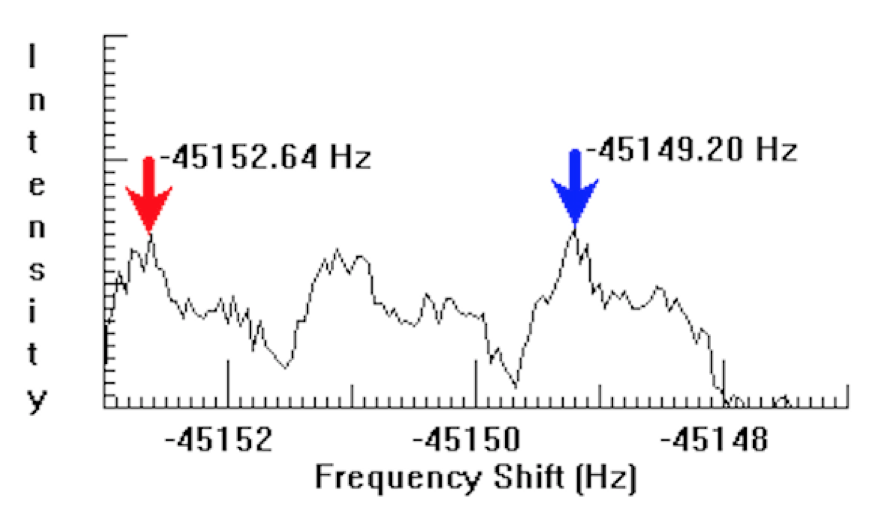
\includegraphics[scale=0.5]{Present_Images.png/1_-_T+390ms.png}
\caption{T+390s interval of the electromagnetic signal from the received pulse.}
\label{1-T+390}
\end{figure}

%-----------------------------------------------------------------------

\subsubsection{Shift in frequency due to rotational velocity}

\begin{equation} \label{eq:7}
{\Delta F_{Total} = \dfrac{F_{Right} - {F_{Left}}}{2}}
\end{equation}\\

Using \cref{eq:7} and the graphs in \cref{Present Graphs} the equations can be filled and the final answer can be produced.

\begin{equation}\label{1-Shift in frequency due to rotational velocity}
\begin{split}
{T+120 = \dfrac{-45150.38 - (-)45151.74}{2}} = 0.68Hz \\
\\
{T+210 = \dfrac{-45149.08 - (-)45151.96}{2}} = 1.44Hz \\
\\
{T+300 = \dfrac{-45148.90 - (-)45152.60}{2}} = 1.85Hz \\
\\
{T+390 = \dfrac{-45149.20 - (-)45152.64}{2}} = 1.72Hz \\
\\
\end{split}
\end{equation}

%-----------------------------------------------------------------------

\subsubsection{Shift in frequency due to echo}

\begin{equation} \label{eq:9}
{\Delta F_{C} = \dfrac{\Delta F_{Total}}{2}}
\end{equation}\\

Using \cref{eq:9} and the answers from \cref{1-Shift in frequency due to rotational velocity} the shift in frequency due to echo can be calculated.

\begin{equation}\label{1-Shift in frequency due to echo}
\begin{split}
{T+120 = \dfrac{0.68}{2}} = 0.34Hz \\
\\
{T+210 = \dfrac{1.44}{2}} = 0.72Hz \\
\\
{T+300 = \dfrac{1.85}{2}} = 0.925Hz \\
\\
{T+390 = \dfrac{1.72}{2}} = 0.86Hz \\
\\
\end{split}
\end{equation}

%-----------------------------------------------------------------------

\subsubsection{Rotational velocity of the edge of Mercury} 

\begin{equation} \label{eq:11}
{V_{0} = c \left(\dfrac{\Delta F_{C}}{f}\right)}
\end{equation}

\begin{equation*}
\begin{split}
&\text{Where;} \\
&\text{Speed of Light} \Rightarrow {c}=3_{\times10^8} \\
&\text{Transmitted Frequency} \Rightarrow {f}=430_{\times10^6} \\
\end{split}
\end{equation*} \\

Using \cref{eq:11} and the answers from \cref{1-Shift in frequency due to echo} the rotational velocity of the edge of Mercury can be calculated.

\begin{equation}\label{1-Rotational velocity of the edge of Mercury}
\begin{split}
{T+120 = 3_{\times10^8} \left(\dfrac{0.34}{430_{\times10^6}}\right)} = 0.237ms^{-1}\\
\\
{T+210 = 3_{\times10^8} \left(\dfrac{0.72}{430_{\times10^6}}\right)} = 0.502ms^{-1}\\
\\
{T+300 = 3_{\times10^8} \left(\dfrac{0.925}{430_{\times10^6}}\right)} = 0.645ms^{-1}\\
\\
{T+390 = 3_{\times10^8} \left(\dfrac{0.86}{430_{\times10^6}}\right)} = 0.600ms^{-1}\\
\\
\end{split}
\end{equation}

%-----------------------------------------------------------------------

\subsubsection{Equatorial velocity of Mercury}

\begin{equation} \label{eq:13}
{V = V_{0} \left(\dfrac{R_{Merc}}{y}\right)}
\end{equation}

\begin{equation*}
\begin{split}
&\text{Where;} \\
&\text{Radius of Mercury} \Rightarrow {R_{Merc}}=2.24_{\times10^6} \\
&\text{Geometrical parameter} \Rightarrow y = \cref{Distance perpendicular to our line of sight equation} \\
\end{split}
\end{equation*} \\

Using \cref{eq:13} and the answers from \cref{1-Rotational velocity of the edge of Mercury} \& \cref{Distance perpendicular to our line of sight equation} the equatorial velocity of Mercury can be calculated.

\begin{equation}\label{1-Equatorial velocity of Mercury}
\begin{split}
{T+120 = 0.237 \left(\dfrac{2.24_{\times10^6}}{294.612_{\times10^3}}\right)} = 1.947ms^{-1} \\
\\
{T+210 = 0.502 \left(\dfrac{2.24_{\times10^6}}{389.189_{\times10^3}}\right)} = 3.121ms^{-1} \\
\\
{T+300 = 0.645 \left(\dfrac{2.24_{\times10^6}}{464.516_{\times10^3}}\right)} = 3.360ms^{-1} \\
\\
{T+390 = 0.600 \left(\dfrac{2.24_{\times10^6}}{528.883_{\times10^3}}\right)} = 2.745ms^{-1} \\
\\
\end{split}
\end{equation}

%-----------------------------------------------------------------------

\subsubsection{Planet rotational period}

\begin{equation} \label{eq:15}
{P_{Rot} =\dfrac{2 \pi R_{Merc}}{V}}
\end{equation}

\begin{equation*}
\begin{split}
&\text{Where;} \\
&\text{Radius of Mercury} \Rightarrow {R_{Merc}}=2.24_{\times10^6} \\
\end{split}
\end{equation*} \\

Using \cref{eq:15} and the answers from \cref{1-Equatorial velocity of Mercury} the rotational period of Mercury can be calculated. \\

\begin{equation} \label{1-Planet rotational period}
\begin{split}
{P_{Rot} =\dfrac{2 * \pi * 2.24_{\times10^6}}{\left(\dfrac{1.947+3.121+3.360+2.745}{4}\right)}} \\
= 5.444_{\times10^6}s \\
= 63.00 Days \\
\end{split}
\end{equation} \\

%-----------------------------------------------------------------------
%	INFERIOR CONJUNCTION
%-----------------------------------------------------------------------

\subsection{Inferior Conjunction}\label{Inferior Conjunction}

Using the same layout of equation to solve the present date stage of this experiment seen in \cref{Present date data} my final answer for the Mercury's rotational period for the inferior conjunction stage of this experiment is;

\begin{equation} \label{2-Planet rotational period}
\begin{split}
{P_{Rot} =\dfrac{2 * \pi * 2.24_{\times10^6}}{\left(\dfrac{2.136+3.146+3.324+2.777}{4}\right)}} \\
= 5.343_{\times10^6}s \\
= 61.84 Days \\
\end{split}
\end{equation} \\

%-----------------------------------------------------------------------
%	GREATEST EASTERN ELONGATION
%-----------------------------------------------------------------------

\subsection{Greatest-Eastern Elongation}\label{Greatest-Eastern Elongation}

Using the same layout of equation to solve the present date stage of this experiment seen in \cref{Present date data} my final answer for the Mercury's rotational period for the greatest-eastern elongation stage of this experiment is;

\begin{equation} \label{3-Planet rotational period}
\begin{split}
{P_{Rot} =\dfrac{2 * \pi * 2.24_{\times10^6}}{\left(\dfrac{3.121+2.991+3.360+2.777}{4}\right)}} \\
= 4.870_{\times10^6}s \\
= 56.37 Days \\
\end{split}
\end{equation} \\

%-----------------------------------------------------------------------
%	ANALYSIS
%-----------------------------------------------------------------------

\subsection{Analysis}

The actual period of rotation of planet Mercury is 58.646 days \cite{The_Solar_System} \\

Analyzing the 3 final results for the rotational period of planet Mercury and comparing them to the actual period of rotation, the result weren't far off but they didn't exactly come close to the actual value. Even though using a simulated software, human error is partly to blame, the equations were double checked but still the underlying physics behind this experiment remain true.

%-----------------------------------------------------------------------
%-----------------------------------------------------------------------
%	CONCLUSION
%-----------------------------------------------------------------------
%-----------------------------------------------------------------------

\section{Conclusion}

To conclude this experiment, using geometry to calculate a planets rotational period is clever even thought the values from this experiment weren't spot on but they were close enough to prove that with exact data the underlying physics in \cref{Physics Behind the Experiment} are true. \\

Using the same value for the transmitted frequency and set geometrical parameter in \cref{Geometrical Parameters} allowed each stage of this experiment to be conducted fairly, thus leaving the only variable in the frequency shift due to rotational velocity in \cref{1-Shift in frequency due to rotational velocity} thus allowing only the position of the planet in orbit of the Sun relative to Earth to be the only deciding factor between all 3 stages of this experiment.

%------------------------------------------------------------------------
%	REFERENCES
%------------------------------------------------------------------------

\end{multicols}
\bibliographystyle{plain}
\bibliography{mybib.bib}

%------------------------------------------------------------------------

\end{document}